\hsection{Installing PyCharm}%
\label{sec:installingPyCharm}%
%
\begin{figure}%
\centering%
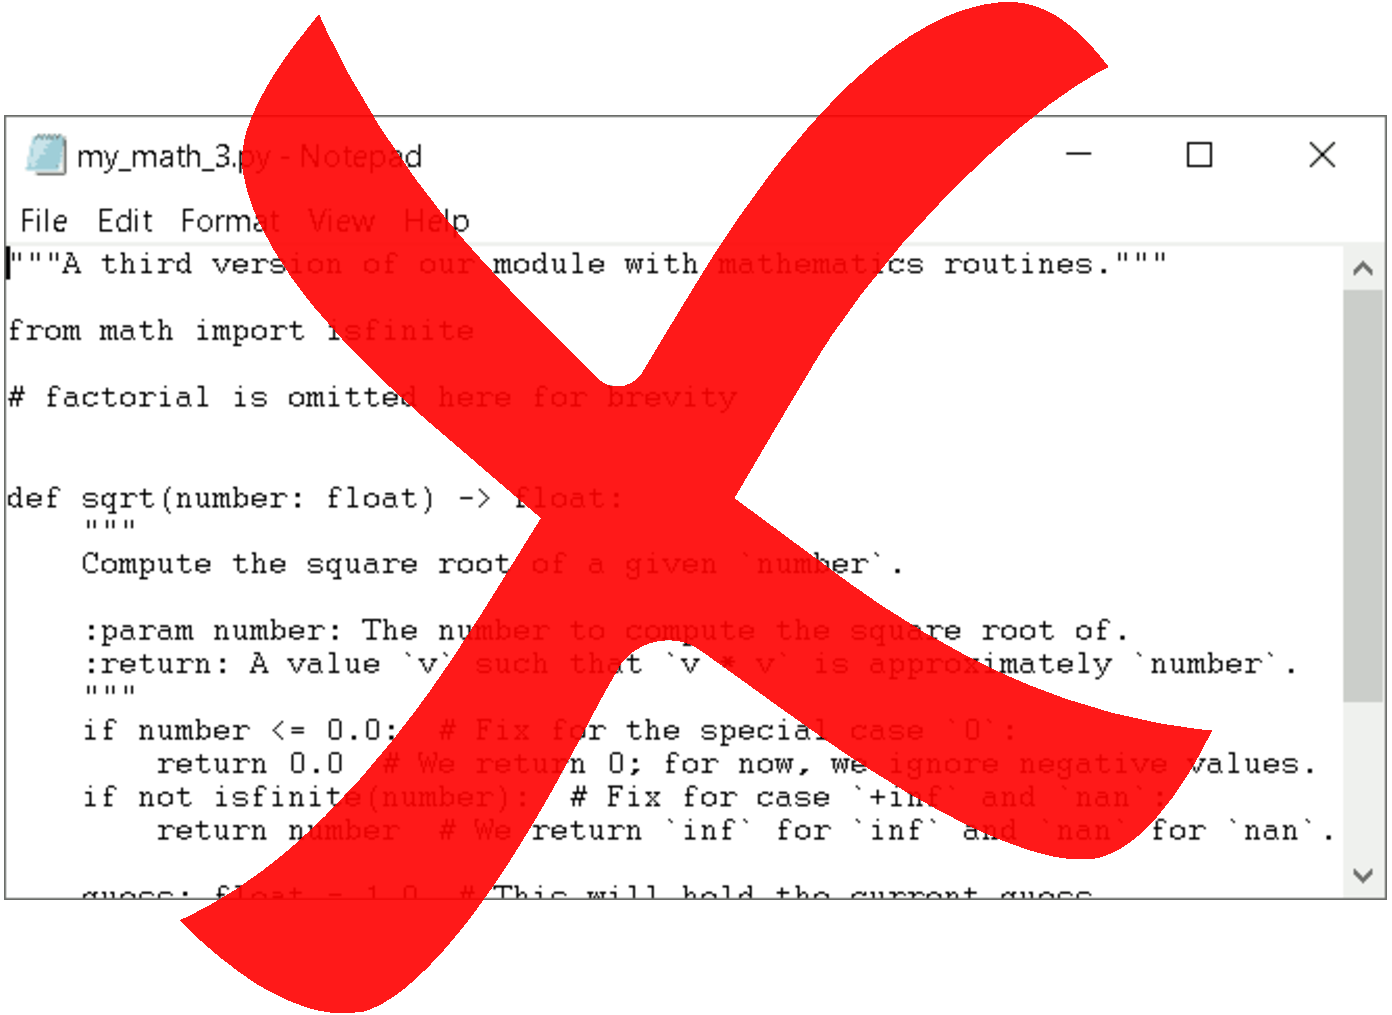
\includegraphics[width=0.5\linewidth]{\currentDir/usingNotepadAsEditor.pdf}%
\caption{We do not want to use the \textil{NotePad}\nobreakdashes-App of \microsoftWindows\ for programming, do we?}%
\label{fig:usingNotepadAsEditor}%
\end{figure}%
%
Just having a programming language and the corresponding interpreter on your system is not enough.
Well, it is enough for just running \python\ programs.
But it is not enough if you want to develop software efficiently.
Are you going to write programs in a simple text editor like a caveperson?
No, of course not, you need an \pgls{ide}, a program which allows you to do multiple of the necessary tasks involved in the software development process under one convenient user interface.
For this book, I recommend using \pycharm~\cite{VHN2023HOADWP,Y2022PPADT,W2024PME}, whose community edition is freely available.
The installation guide for \pycharm\ can be found at \url{https://www.jetbrains.com/help/pycharm/installation-guide.html}.%
%
\hinput{installingPyCharmUbuntu}{installingPyCharmUbuntu}%
\hinput{installingPyCharmWindows}{installingPyCharmWindows}%
\endhsection%
%
